%% Paste this BODY into the official ML4H 2026 Overleaf template.
%% Keep the template preamble / .sty. Do not use the local article preamble.
%% Put these four macros in the template preamble (before \begin{document}):
%%   \newcommand{\yes}{\textsf{yes}}
%%   \newcommand{\no}{\textsf{no}}
%%   \newcommand{\maybe}{\textsf{maybe}}
%%   \newcommand{\uscore}{$u$-score}
%% Then: upload sections/, figures/*.pdf, references.bib.

\title{When the Signal Isn't in the Text:\\
Nine Signals and Debate Fail to Recover PubMedQA maybe}
\author{Anonymous Author(s)\\
\textit{Affiliation withheld for review}}
\date{}

% --- after \begin{document} \maketitle of the official template ---

\begin{abstract}
Nine uncertainty signals and compute-matched debate fail to recover
PubMedQA \maybe{}; the deliverable is coverage-constrained abstention,
not retrieval or multi-agent accuracy. On PQA-L $500$, hit@1 is $0.980$
$[0.968,0.992]$ (citation-support $1.000$) because gold is the source
abstract; BioLinkBERT reaches only $0.726$ $[0.688,0.764]$. Eight of
nine headline AUROC CIs include $0.5$ (\texttt{gpt-5} $0.554$). On the
same $90$ IDs, ungated debate is identical to BioLinkBERT ($0.656$
$[0.556,0.744]$, $0$ discordant pairs) and compute-matched
self-consistency ($N{=}8$, $8.0$ LLM calls/case) is $0.522$
$[0.422,0.622]$. Selective prediction cuts expected cost $-16.4\%$
versus always-answer $0.356$ at $\ge 50\%$ coverage (AURC $0.311$,
unanchored vs.\ a ranker).
\end{abstract}

\noindent{\small \textbf{Keywords:} abstention, selective prediction, uncertainty,
PubMedQA, negative result}

\noindent{\small \textbf{Data and Code Availability.}
Official PubMedQA PQA-L~\citep{jin2019pubmedqa} (public). Per-case signals,
bootstrap statistics (\texttt{statistics.json}), and figure scripts ship as
anonymized supplemental material. No deanonymizing repository URL at review.
Upon acceptance we will release evaluation scripts and reports.
\textbf{IRB.} Public research abstracts and official labels only; no
patient-identifiable records collected. No live human-subjects study was
run. Control C3 uses the official PubMedQA single-annotator labels as a
proxy, not a new annotation. No IRB approval is required.
\textbf{Publication Ethics / LLM use.} Debate, audit, and self-consistency
calls are part of the method; the authors take responsibility for all
reported numbers and the bibliography. The manuscript and evaluation
scripts were drafted with AI writing/coding assistance; every claim was
checked against the released JSON.}

\section{Introduction}
\label{sec:intro}

A system that answers a question the evidence cannot support is worse
than one that declines. PubMedQA~\citep{jin2019pubmedqa} operationalises
that requirement: given a research question and the abstract that
motivated it, the label is \yes{}, \no{}, or \maybe{} --- and \maybe{}
means \emph{inconclusiveness}, not a third topic.

Headline accuracies of $\sim$78--84\% are driven by \yes{}/\no{}.
Replacing an LLM judge with calibrated
BioLinkBERT~\citep{yasunaga2022linkbert} raised label accuracy from
$0.536$ to $0.726$ $[0.688,0.764]$ on the same PQA-L $500$ run; hit@1
stayed $0.980$. That near-ceiling is expected: gold is the source
abstract in a $500$-abstract corpus, so retrieval contributes nothing;
the gap is that the abstract does not decide the label. \maybe{} recall
is still only $0.073$ ($4/55$; Figure~\ref{fig:stages}).

We measure nine uncertainty signals, a compute-matched debate, and a
fixed DeBERTa-NLI auditor~\citep{abdaljalil2026knowing}. The findings
are consistently negative, and that is the result. Across judges and
signals, \maybe{} is statistically indistinguishable from chance in the
abstract (Figure~\ref{fig:forest}). Three controls localise the cause:
(C1)~the NLI auditor is at chance (AUROC $0.497$); (C2)~giving the
authors' gold conclusion lifts \texttt{gpt-5} only to $0.592$ (CI still
includes $0.5$); (C3)~the official PubMedQA single annotator reaches
$0.60$ \maybe{} recall versus $\approx 0$ for every model ($p{=}0.0002$)
yet still errs on $40\%$. Relative to \citet{lionetti2025clinical}
(ML4H 2025 Findings: uncertain labels) and \citet{tramontini2026rag}
(ML4H 2025 Proceedings: abstention in trial matching), this is a
complementary PubMedQA regime: inconclusiveness is often not in the
text, so the practice question is when to refuse.

We therefore treat the deliverable as \emph{selective prediction}, not
recovered \maybe{} accuracy. On the same $90$ IDs, ungated debate is
identical to the classifier ($0.656$ $[0.556,0.744]$, $0$ discordant,
McNemar $p{=}1$) --- a collapse control, not a second system --- and
compute-matched SC is $0.522$ $[0.422,0.622]$ at $8$ LLM calls each
(Section~\ref{sec:experiments}).

\noindent\textbf{Contributions.}
(1)~A complementary PubMedQA regime vs.\ Lionetti and Tramontini:
inconclusiveness often is not in the text; the practice question is
when to refuse.
(2)~A negative result: nine headline signals, four judges including
\texttt{gpt-5}, bootstrap CIs, official single-annotator control C3, and
seven-seed routing instability --- \maybe{} is not recoverable from the
abstract.
(3)~Coverage-constrained abstention: a $16.4\%$ expected-cost cut
versus always-answer $0.356$ at $\ge 50\%$ coverage on $n{=}90$ (AURC
$0.311$ is unanchored vs.\ a ranker), with all artefacts released.

\section{Related Work}
\label{sec:related}

Multi-agent debate was introduced to improve
factuality~\citep{du2023debate} and adopted in medicine
\citep{tang2024medagents,kim2024mdagents,chen2024reconcile}, yet
compute-matched controls and MedAgentBoard find it rarely beats a
strong single model~\citep{wang2023selfconsistency,smit2024mad,choi2025debate,zhang2025stop,zhu2025medagentboard}.
We measure the same collapse on PubMedQA \maybe{} (unanimous on $93\%$
of true-\maybe{} cases). Selective prediction~\citep{elyaniv2010foundations}
lets a model abstain; MedQAbstain~\citep{cocchieri2026llms} shows LLMs
almost never do on medical MCQA, and a fixed NLI
auditor~\citep{abdaljalil2026knowing} is AUROC $0.497$ here (C1).
\citet{lionetti2025clinical} (ML4H 2025 Findings) treat clinical labels
as uncertain; \citet{tramontini2026rag} (Proceedings 2025) study
abstention in trial matching; SCARE~\citep{lee2026scare} classifies
SQL/EHR answerability --- complementary PubMedQA work asks whether the
abstract is conclusive. Semantic entropy~\citep{kuhn2023semantic}
assumes recoverability from the input; \maybe{} tests the opposite.

\section{Method}
\label{sec:method}

Three layers share one LLM backend. Debate is a collapse control
(identical to BioLinkBERT, $0$ discordant, $n{=}90$), not an
architectural contribution; the panel score \uscore{} and a calibrated
router remain. An NLI auditor and a gold-conclusion oracle are
controls, not accuracy boosters.

\begin{figure}[t]
  \centering
  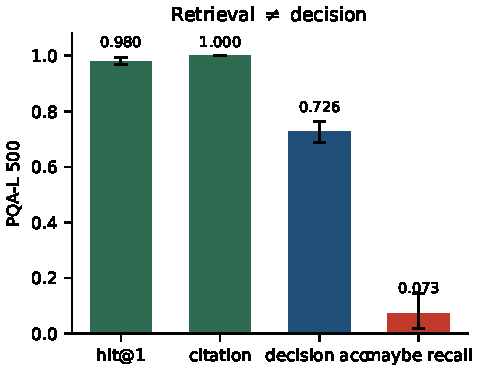
\includegraphics[width=\columnwidth]{figures/stage_separated.pdf}
  \caption{Stage-separated metrics on PQA-L $500$ ($95\%$ CI). Retrieval
  (hit@1 $0.980$, citation $1.000$) and BioLinkBERT decision ($0.726$) do not
  overlap; \maybe{} recall is $0.073$. Source: supplemental
  \texttt{statistics.json}.}
  \label{fig:stages}
\end{figure}

\paragraph{Debate.}
Debate is a collapse control, not an architectural contribution: on
$n{=}90$ ungated debate is identical to BioLinkBERT ($0.656$
$[0.556,0.744]$, $59/90$, $0$ discordant pairs). We run supervisor-free
round-robin (\texttt{round\_robin\_no\_supervisor}): round~1 independent;
rounds~2--3 sequential with peer context; four personas including an
\emph{uncertainty advocate}. Each opinion emits a label,
\texttt{evidence\_conclusiveness}, and a confidence; a two-step rule
assigns \maybe{} when Step~1 is inconclusive.

\paragraph{BioLinkBERT gate.}
A calibrated BioLinkBERT-large classifier is the decision baseline
($0.726$ on PQA-L $500$). A confident ($\ge 0.90$) hard \yes{}/\no{} is
trusted unless the panel is unanimous on the opposite hard label.
Among errors on gold \maybe{}, $21/26$ mispredictions on
\texttt{balanced90} had confidence $\ge 0.90$, so threshold gating
cannot recover abstention. Panel majority without the gate (round-1
vote) is $0.567$ $[0.467,0.667]$ on the same IDs.

\paragraph{\uscore{} and routing.}
$u=\mathrm{clip}_{[0,1]}(\sum_k w_k f_k)$ over label entropy, \maybe{} and
inconclusive fractions, disagreement, flip rate, semantic
entropy~\citep{kuhn2023semantic}, a BioLinkBERT-is-\maybe{} bit, and an optional
audit score. \texttt{calibrate\_threshold} sweeps $t$ on a held-out split
(default macro-$F_1$) and routes to \maybe{} iff $u\ge t$. On this run
routing is not the primary accuracy: held-out $n{=}45$ drops ungated
$0.644$ to $0.622$. We report the risk--coverage curve, AURC, and a
cost-sensitive analysis (wrong${=}1.0$, abstain${=}0.25$) with a
$\ge 0.5$ coverage constraint.

\paragraph{Auditors.}
The generative auditor decomposes the question into 2--4 checkable conditions
(\texttt{supported}/\texttt{refuted}/\texttt{silent}). The external auditor is
fixed \texttt{cross-encoder/nli-deberta-v3-base}: high score when the abstract
is neutral to both polarities~\citep{abdaljalil2026knowing}.

\section{Experimental Setup}
\label{sec:experiments}

\paragraph{Data.}
Official PubMedQA PQA-L~\citep{jin2019pubmedqa}. Full-scale metrics use PQA-L
$500$ ($276$~\yes{}, $169$~\no{}, $55$~\maybe{}). Signal AUROC uses
\texttt{balanced90} ($30$ each) so \maybe{}-vs-rest has $30$ positives.

\paragraph{Pinned models.}
Debate and generative audit: \texttt{qwen2.5:7b} (primary),
\texttt{qwen2.5:14b}, \texttt{deepseek-r1:14b}. Flagship control:
\texttt{gpt-5} (OpenAI API). Decision classifier: BioLinkBERT-large, pinned
checkpoint \texttt{pubmedqa\_biolinkbert\_seed47} (training seed $47$). External auditor:
\texttt{cross-encoder/nli-deberta-v3-base}. Retrieval: MedCPT (dense) $+$ BM25
$+$ MedCPT cross-encoder reranker. Debate uses $T{=}0.3$; SC uses $T{=}0.7$
because sample diversity \emph{is} the SC mechanism. Frozen abstract for
both generative arms. LLM calls (debate, audit, SC) are part of the
method; authors take responsibility for the numbers they produce.

\paragraph{Metrics.}
AUROC (\maybe{} vs rest) with $95\%$ bootstrap CIs ($5000$ resamples, seed
$47$). Human comparison: \maybe{} recall, bootstrap difference CI, permutation
$p$. Selective prediction: risk--coverage, AURC, expected cost with
$\ge 0.5$ coverage. Routing stability: seven calibration seeds.

\paragraph{Controls.}
C1: swap the generative auditor for DeBERTa-NLI. C2: feed the authors'
\texttt{long\_answer} instead of the abstract. C3: official PubMedQA
single-annotator labels on \texttt{balanced90} (a proxy; no new
human-subjects study).

\paragraph{Self-consistency.}
The compute-matched control is $N{=}8$ independent \texttt{generalist}
samples, majority vote, frozen abstract, \texttt{qwen2.5:7b}. $N$ equals
\texttt{mean\_llm\_calls\_per\_case}${}=8.0$ from the instrumented debate
run on the same $90$ IDs (both arms: $720$ calls, $0$ failures). Primary
debate metric is ungated \texttt{bert\_gate} on all $90$, not the routed
held-out $n{=}45$ summary. Debate does not beat BioLinkBERT; SC is worse
on the point estimate and is not a significant difference.

\section{Results}
\label{sec:results}

\paragraph{Retrieval $\neq$ decision.}
Figure~\ref{fig:stages} separates the stages on
PQA-L $500$. Hit@1 is $1$ iff the gold source PMID --- the PubMedQA
source abstract the question was written from --- is the top-1 hit in
the official $500$-abstract corpus; citation-support passes iff every
inline $[S\#]$ cites a retrieved document in canonical form (structural
validation, not claim-level entailment). Hit@1 $=$ hit@3 $=0.980$
$[0.968,0.992]$; citation-support is $1.000$. That near-ceiling is
expected on this construction; the decision is the gap. Headline
BioLinkBERT accuracy is $0.726$ $[0.688,0.764]$ on $n{=}500$ (LLM judge
on the same run: $0.536$; hit@1 unchanged), not the diagnostic-split
$0.656$ $[0.556,0.744]$ on \texttt{balanced90}. The intervals do not
overlap retrieval. \maybe{} recall is $0.073$ $[0.018,0.145]$: only
$23/500$ predicted \maybe{} against $55$ gold ($26$ collapsed to
\yes{}, $25$ to \no{}). On \texttt{balanced90} the same checkpoint has
\maybe{} recall $0.133$ ($4/30$). The evidence is found; it does not
decide the question.

\paragraph{Compute-matched debate vs.\ SC, same $90$ IDs.}
Table~\ref{tab:stages} is the inviolable comparison. Ungated debate
(\texttt{bert\_gate}, \texttt{qwen2.5:7b}, frozen abstract) is
identical to BioLinkBERT: $0.656$ $[0.556,0.744]$ ($59/90$),
$0$ discordant pairs, McNemar $p{=}1$, \maybe{} recall $0.133$. We
report that collapse, not a second competing system. The panel without
the gate --- round-1 majority vote, no BioLinkBERT --- is $0.567$
$[0.467,0.667]$ ($51/90$) on the same IDs. Compute-matched SC ($N{=}8$,
$8.0$ LLM calls/case, $T{=}0.7$ vs.\ debate $T{=}0.3$) is $0.522$
$[0.422,0.622]$ ($47/90$); its higher \maybe{} recall $0.567$ ($17/30$)
comes from over-predicting \maybe{} ($45/90$). Matched $8$ calls,
debate still spends ${\sim}10.6$k tokens/case versus SC ${\sim}8.0$k
--- no accuracy win over BERT on the same $90$ IDs. McNemar exact
$p{=}0.088$ (debate vs.\ SC; $27$ vs.\ $15$ discordant) is a
point-estimate gap only. Routing is not primary: on the held-out $45$ it drops ungated
$0.644$ to $0.622$ (SC on those IDs is $0.533$). $95\%$ CIs on
$n{=}90$ are case-level bootstrap ($5000$ resamples, seed $47$) from
the per-case labels in the two JSON reports.

\begin{table}[t]
\centering
\caption{Decision accuracy. Headline BioLinkBERT is $0.726$ on PQA-L $500$.
Apples-to-apples rows share the same $90$ IDs, frozen abstract,
\texttt{qwen2.5:7b}. Debate ungated is \texttt{bert\_gate} --- identical
to BERT, not a second system. Panel maj.\ is round-1 majority without
BERT. $n{=}90$ CIs: case bootstrap, $5000$ resamples, seed $47$.
Routed held-out $n{=}45$ accuracy $0.622$ is \emph{not} primary.$^\dagger$}
\label{tab:stages}
{\scriptsize
\begin{tabular}{@{}lcccc@{}}
\toprule
System & Acc. & $95\%$ CI & $n$ & Calls \\
\midrule
BERT (PQA-L $500$) & $0.726$ & $[0.688,0.764]$ & $500$ & --- \\
BERT (bal.\ $90$) & $0.656$ & $[0.556,0.744]$ & $90$ & --- \\
Debate ungated & $0.656$ & $[0.556,0.744]$ & $90$ & $8.0$ \\
Panel maj.\ (no BERT) & $0.567$ & $[0.467,0.667]$ & $90$ & $8.0$ \\
SC ($N{=}8$) & $0.522$ & $[0.422,0.622]$ & $90$ & $8.0$ \\
\bottomrule
\end{tabular}}
\\[0.25em]
{\scriptsize $^\dagger$Routed debate on held-out $45$: $0.622$ (drop from
ungated $0.644$ on those IDs; SC $0.533$). McNemar debate vs.\ BERT: $0$
discordant, $p{=}1$. Debate vs.\ SC: $p{=}0.088$ --- point estimate only.}
\end{table}

\paragraph{No uncertainty signal beats chance.}
Figure~\ref{fig:forest} collects \maybe{}-vs-rest AUROC on
\texttt{balanced90}. Point estimates sit in $0.46$--$0.62$. Nine
headline signals are reported ($u$-score, four generative audits,
DeBERTa-NLI, two gold-conclusion oracles, plus the NLI oracle). Eight of
nine $95\%$ CIs include $0.5$, including \texttt{gpt-5} ($0.554$
$[0.429,0.678]$) and DeBERTa-NLI ($0.497$ $[0.363,0.632]$). The only
interval that clears $0.5$ is the \texttt{qwen2.5:14b} gold-conclusion
oracle ($0.622$ $[0.501,0.737]$), and it barely does. The
\texttt{gpt-5} oracle is $0.592$ $[0.463,0.714]$ --- still chance.

\begin{figure}[t]
  \centering
  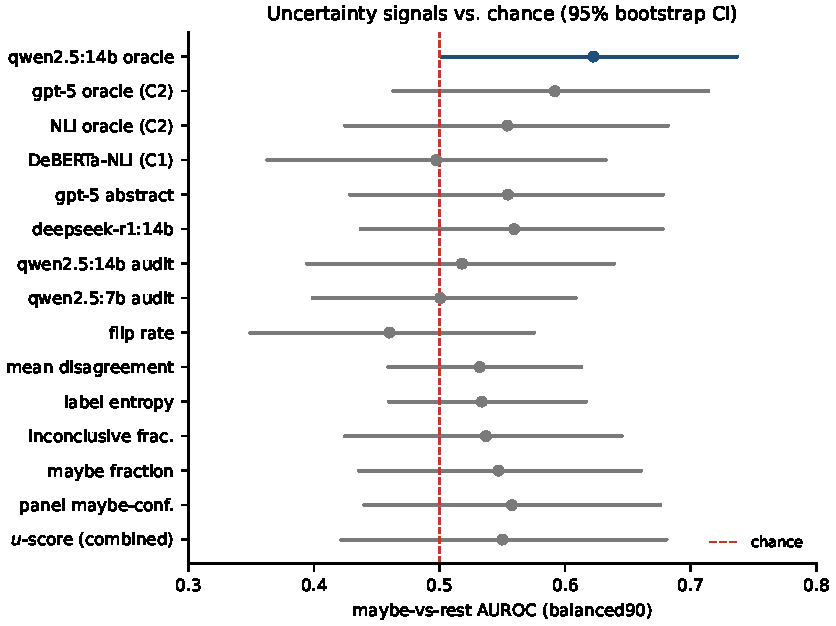
\includegraphics[width=\columnwidth]{figures/auroc_forest.pdf}
  \caption{\maybe{}-vs-rest AUROC, \texttt{balanced90}, $5000$ bootstrap
  resamples (seed $47$). Grey: CI includes $0.5$. Navy: sole interval
  that excludes chance (\texttt{qwen2.5:14b} gold-conclusion oracle).
  Eight of nine headline CIs include $0.5$. Source: supplemental
  \texttt{statistics.json}.}
  \label{fig:forest}
\end{figure}

\paragraph{Official annotator beats models; the residual is partly irreducible.}
Official single-annotator predictions (C3) on \texttt{balanced90}:
\maybe{} recall $0.60$ (accuracy $0.800$, $\kappa{=}0.70$) versus
$\approx 0.00$ for every model signal. Difference $0.60$, $95\%$ CI
$[0.43,0.77]$, permutation $p{=}0.0002$. Giving C3 the gold
\texttt{long\_answer} lowers overall accuracy $0.800{\to}0.711$ while
\maybe{} recall only moves $0.60{\to}0.63$.

\paragraph{Routing is unstable; selective prediction still pays.}
Seven-seed routing (macro-$F_1$) yields accuracy $0.587\pm 0.075$ and
\maybe{} recall $0.257\pm 0.144$ (range $[0.067,0.467]$). The spread is
evidence that the signal is too weak to tune. Nonetheless the
risk--coverage AURC is $0.311$ (Figure~\ref{fig:risk}). No random or
BERT-confidence AURC is in the released analysis files, so $0.311$ is
unanchored as a ranker comparison; we treat always-answer expected cost
$0.356$ ($n{=}90$) as the operating-point anchor. Unconstrained cost
optimisation degenerates to abstain-on-everything. The constrained
point --- answer at least half of cases --- cuts expected cost from
$0.356$ to $0.297$ ($-16.4\%$) at $52\%$ coverage
(Table~\ref{tab:cost}). Always-answer $0.356$ is not
$1-0.656{=}0.344$: a predicted \maybe{} is charged as abstention
($0.25$), so $31$ errors and $4$ correct \maybe{}s give
$(31{+}1)/90{=}0.356$.

\begin{figure}[t]
  \centering
  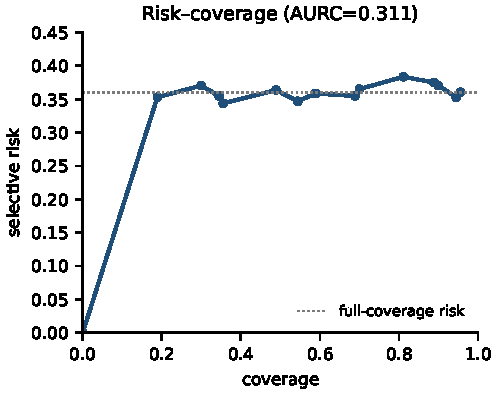
\includegraphics[width=\columnwidth]{figures/risk_coverage.pdf}
  \caption{Risk--coverage for the routed \uscore{} on \texttt{balanced90}
  ($n{=}90$). AURC $0.311$ (no ranker baseline in the released files).
  The usable operating point is constrained $\ge 50\%$ coverage
  (Table~\ref{tab:cost}), not unconstrained abstain-all.}
  \label{fig:risk}
\end{figure}

\begin{table}[t]
\centering
\caption{Cost-sensitive selective prediction on $n{=}90$
(wrong${=}1.0$, abstain${=}0.25$). A predicted \maybe{} costs $0.25$,
so always-answer is $0.356$, not the $0$-$1$ error rate $0.344$.}
\label{tab:cost}
{\scriptsize
\begin{tabular}{@{}lcccc@{}}
\toprule
Point & Cost & Abstain & $n$ & vs always \\
\midrule
Always answer & $0.356$ & $0\%$ & $90$ & --- \\
Unconst.\ opt. & $0.250$ & $100\%$ & $90$ & $-29.7\%$ (deg.) \\
$\ge 50\%$ cov. & $0.297$ & $48\%$ & $90$ & $\mathbf{-16.4\%}$ \\
\bottomrule
\end{tabular}}
\end{table}

\section{Discussion}
\label{sec:discussion}

The deciding information for many PubMedQA \maybe{} items is not in the
abstract the model reads. The failure is invariant to the answering
procedure (nine headline signals, four judges, a dedicated NLI auditor).
It is not retrieval (hit@1 $0.98$ on a source-abstract gold; CIs do not
overlap decision accuracy). Injecting the gold conclusion moves the best
oracle only to $0.62$, and the official single annotator (C3) still errs
on $40\%$. Others improve \emph{how} a model
answers~\citep{abdaljalil2026knowing,cocchieri2026llms,wynn2025talk};
here the problem is upstream.

We do not claim SOTA or that debate improves anything. Ungated debate is
identical to BioLinkBERT ($0.656$ $[0.556,0.744]$, $0$ discordant,
McNemar $p{=}1$). SC is lower at matched compute ($0.522$
$[0.422,0.622]$); McNemar $p{=}0.088$ is not a significance claim.
Routed debate ($0.622$ on held-out $45$) is not primary. NLI AUROC
$0.497$ is a control failure. Limits: debate/SC were not run on PQA-L
$500$; one benchmark; contamination is possible; \texttt{bert\_gate} is
a BERT copy and the panel-only majority is $0.567$; C3 is the official
single annotator, not a new multi-rater study; $\ge 70$B open models
were not run.

The $-16.4\%$ figure is a coverage-constrained cost cut versus
always-answer on $n{=}90$, not a ranker-anchored AURC win and not a
bedside claim. SCARE~\citep{lee2026scare} and
FHIR-AgentBench~\citep{lee2026fhir} ask SQL/EHR answerability; we ask
whether the abstract is conclusive. The symposium argument is label
versus abstain, not a new architecture. Per-case signals and statistics
ship as anonymized supplemental material.


\bibliography{references}
